%%%%%%%%%%%%%%%%%%%%%%%%%%%%%%%%%%%%%%%%%
% Jacobs Portrait Poster
% LaTeX Template
% Version 1.0 (31/08/2015)
% (Based on Version 1.0 (29/03/13) of the landscape template
%
% Created by:
% Computational Physics and Biophysics Group, Jacobs University
% https://teamwork.jacobs-university.de:8443/confluence/display/CoPandBiG/LaTeX+Poster
% 
% Further modified by:
% Nathaniel Johnston (nathaniel@njohnston.ca)
%
% Portrait version by:
% John Hammersley
%
% The landscape version of this template was downloaded from:
% http://www.LaTeXTemplates.com
%
% License:
% CC BY-NC-SA 3.0 (http://creativecommons.org/licenses/by-nc-sa/3.0/)
%
%%%%%%%%%%%%%%%%%%%%%%%%%%%%%%%%%%%%%%%%%

%----------------------------------------------------------------------------------------
%	PACKAGES AND OTHER DOCUMENT CONFIGURATIONS
%----------------------------------------------------------------------------------------

\documentclass[final]{beamer}

\usepackage[scale=1]{beamerposter} % Use the beamerposter package for laying out the poster
\usepackage{xcolor}
\usepackage{amsmath}
\usepackage{amssymb}
\usepackage{siunitx}
\usepackage{braket}
\usepackage{bbold}
\usepackage{bigints}
\usepackage{mathtools}
\usepackage{bm}

\sisetup{detect-all,mode=math,math-rm=\mathrm}

\definecolor{ubcblue}{cmyk}{1,0.9,0.13,0.68}
\definecolor{ubcblue1}{cmyk}{1,0.68,0.04,0}
\definecolor{ubcblue2}{cmyk}{0.8,0.12,0.01,0}
\definecolor{ubcblue3}{cmyk}{0.64,0.1,0.01,0}
\definecolor{ubcblue4}{cmyk}{0.52,0.05,0.03,0}
\definecolor{ubcblue5}{cmyk}{0.38,0.02,0.05,0}

\usetheme{confposter} % Use the confposter theme supplied with this template

\setbeamercolor{block title}{fg=ubcblue,bg=white} % Colors of the block titles
\setbeamercolor{block body}{fg=black,bg=white} % Colors of the body of blocks
\setbeamercolor{block alerted title}{fg=white,bg=ubcblue} % Colors of the highlighted block titles
\setbeamercolor{block alerted body}{fg=black,bg=white} % Colors of the body of highlighted blocks
% Many more colors are available for use in beamerthemeconfposter.sty

%-----------------------------------------------------------
% Define the column widths and overall poster size
% To set effective sepwid, onecolwid and twocolwid values, first choose how many columns you want and how much separation you want between columns
% In this template, the separation width chosen is 0.024 of the paper width and a 4-column layout
% onecolwid should therefore be (1-(# of columns+1)*sepwid)/# of columns e.g. (1-(4+1)*0.024)/4 = 0.22
% Set twocolwid to be (2*onecolwid)+sepwid = 0.464
% Set threecolwid to be (3*onecolwid)+2*sepwid = 0.708

\newlength{\sepwid}
\newlength{\onecolwid}
\newlength{\twocolwid}
\newlength{\threecolwid}
\setlength{\paperwidth}{36in} % A0 width: 46.8in
\setlength{\paperheight}{48in} % A0 height: 33.1in
\setlength{\sepwid}{0.024\paperwidth} % Separation width (white space) between columns
%\setlength{\onecolwid}{0.22\paperwidth} % Width of one column
%\setlength{\twocolwid}{0.464\paperwidth} % Width of two columns
%\setlength{\threecolwid}{0.708\paperwidth} % Width of three columns
\setlength{\onecolwid}{0.3013\paperwidth} % Width of one column
\setlength{\twocolwid}{0.6267\paperwidth} % Width of two columns
\setlength{\topmargin}{-0.5in} % Reduce the top margin size
%-----------------------------------------------------------

\usepackage{graphicx}  % Required for including images

\usepackage{booktabs} % Top and bottom rules for tables
\usepackage{eso-pic}

%----------------------------------------------------------------------------------------
%	TITLE SECTION 
%----------------------------------------------------------------------------------------

\title{Incoherent tunneling and topological \\superconductivity in twisted cuprate bilayers}

\author{\underline{Rafael Haenel}\inst{1,2}, Tarun Tummuru\inst{1,3}, Marcel
Franz\inst{1}}

\institute{
	\inst{1} Department of Physics and Astronomy \& Stewart Blusson Quantum
	Matter Institute, University of British Columbia \\
	\inst{2} Max Planck Institute for Solid State Research \quad
\inst{3} Department of Physics, University of Zurich}
%----------------------------------------------------------------------------------------

\usepackage{exscale}
\begin{document}

\newcommand\AtPagemyLowerLeft[1]{\AtPageLowerLeft{%
\put(\LenToUnit{0.805\paperwidth},\LenToUnit{0.957\paperheight}){#1}}}
\newcommand\AtPagemyLowerRight[1]{\AtPageLowerLeft{%
\put(\LenToUnit{0.014\paperwidth},\LenToUnit{0.953\paperheight}){#1}}}
\AddToShipoutPictureFG{
  \AtPagemyLowerLeft{{
\includegraphics[width=17cm,keepaspectratio]{fig/logos3}}}
}%
\AddToShipoutPictureFG{
	\AtPagemyLowerRight{{
\includegraphics[width=10.5cm,keepaspectratio]{fig/ubc_qmi}}}
}%


\addtobeamertemplate{block end}{}{\vspace*{2ex}} % White space under blocks
\addtobeamertemplate{block alerted end}{}{\vspace*{2ex}} % White space under highlighted (alert) blocks

\setlength{\belowcaptionskip}{2ex} % White space under figures
\setlength\belowdisplayshortskip{2ex} % White space under equations

\begin{frame}[t] % The whole poster is enclosed in one beamer frame

\begin{columns}[t] % The whole poster consists of three major columns, the second of which is split into two columns twice - the [t] option aligns each column's content to the top

\begin{column}{\sepwid}\end{column} % Empty spacer column

\begin{column}{\onecolwid} % The first column

%----------------------------------------------------------------------------------------
%	OBJECTIVES
%----------------------------------------------------------------------------------------

\begin{alertblock}{Summary}
We assess the influence of incoherent tunneling on the phase diagram of a
twisted cuprate bilayer, previously shown to engender a chiral topological state
with spontaneously broken time-reversal symmetry $\mathcal{T}$ in the absence of
incoherence. We show that the
bilayer system continues to support a fully gapped topological phase, even in the limit
of strong disorder-mediated interlayer coupling.
\end{alertblock}

%----------------------------------------------------------------------------------------
%	INTRODUCTION
%----------------------------------------------------------------------------------------


\begin{block}{Introduction}

\begin{figure}
	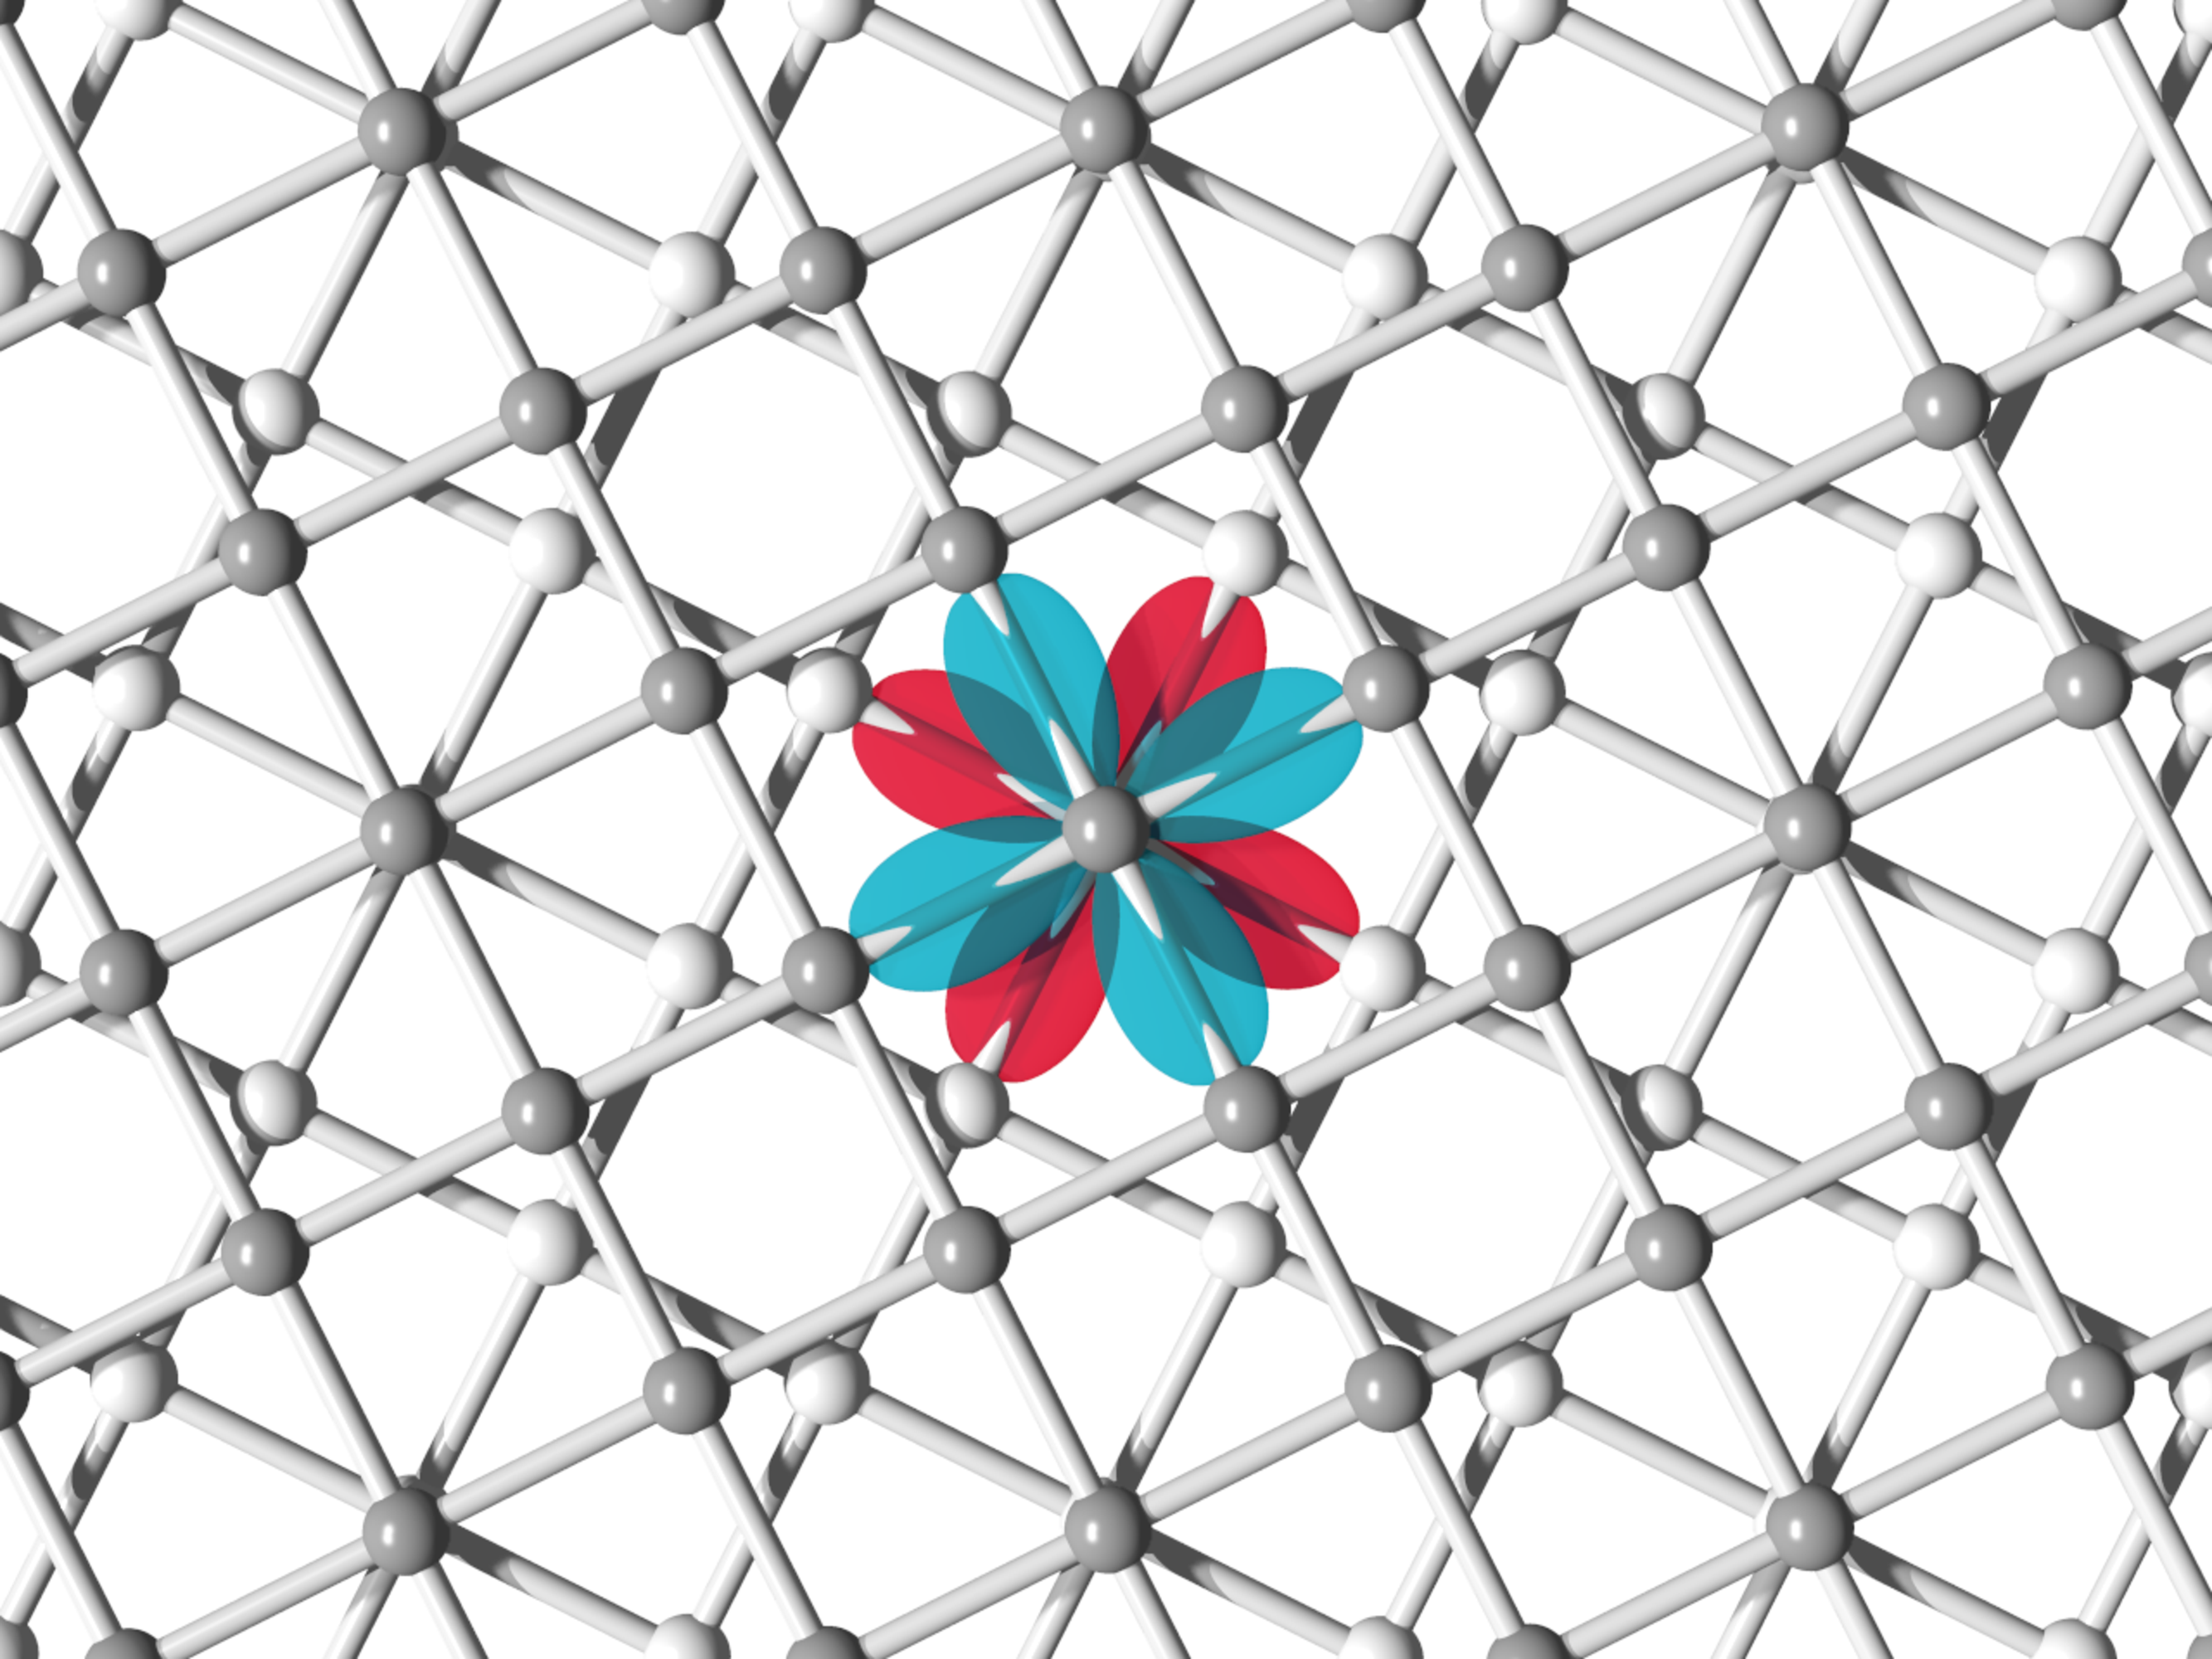
\includegraphics[width=0.7\linewidth]{fig/fig0}
\label{fig:twist}
\end{figure}

A pair of cuprate monolayers, stacked and twisted to $45^\circ$,
spontaneously breaks time-reversal symmetry $\mathcal{T}$
\cite{Can2021}. This can be understood from a Landau-Ginzburg theory \cite{Annett1990}
with two order parameters $\Psi_i e^{\pm i \varphi/2}$ and free energy
\begin{align}
    \mathcal{F}(\varphi) = -B \,  \Psi_1^2\Psi_2 \cos \varphi + C \, \Psi_1
    \Psi_2^2 \cos 2\varphi \,.
    \label{eq:LG}
\end{align}

At $45^\circ$ twist, the point group changes from $D_4$ to $D_{4d}$ with the
additional symmetry element in the $d$-wave $E_2$ irrep
$$S_8: (\Psi_1,\Psi_2)\rightarrow (\Psi_2,-\Psi_1)$$ 
that only leaves the $\cos 2\varphi$ term in Eq.~\ref{eq:LG} invariant.
Thus, the free energy becomes 
$ \mathcal{F}(\varphi) = C \, \Psi_1^2
\Psi_2^2 \cos 2\varphi $ whose minima spontaneously break $\mathcal{T}$ for
$C>0$.

\vspace{0.8cm}

\begin{center}
\begin{tabular}{ c c c c c c c }
	\hline
	$D_{4}$ & Basis functions & $E$ & $2C_4$ & $C_2$ & $2C_2'$ &
	$2C_2''$ \\
	\hline
	A$_{1}$ & $1$ & 	1&1&1&1&1\\
	A$_{2}$ &  & 	1&1&1&-1&-1\\
	B$_{1}$ & $x^2-y^2$ & 		1&-1&1&1&-1\\
	B$_{2}$ & $xy$ & 		1&-1&1&-1&1\\
	E & $(x,y)$ & 			2&0&-2&0&0\\
	\hline
\end{tabular}
\end{center}

\vspace{1cm}

\begin{center}
\begin{tabular}{ c c c c c c c c c }
	\hline
	$D_{4d}$ & Basis functions & $E$ & $2S_8$ & $2C_4$ & $2S_8^3$ &
	$C_2$ & $4C_2'$ & $4\sigma_d$ \\
	\hline
	A$_{1}$ & $1$ & 	1&1&1&1&1&1&1 \\
	A$_{2}$ &  & 		1&1&1&1&1&-1&-1 \\
	B$_{1}$ & $(x^2-y^2)^2-4x^2y^2$ & 		1&-1&1&-1&1&1&-1 \\
	B$_{2}$ & $xy(x^2-y^2)$ & 		1&-1&1&-1&1&-1&1 \\
	E$_1$ & $(x,y)$ & 		2&\sqrt{2}&2&-\sqrt{2}&-2&0&0 \\
	E$_2$ & $(x^2-y^2,xy)$ & 	2&0&-2&0&2&0&0 \\
	E$_3$ & $(y(3x^2-y^2),x(x^2-3y^2))$ & 		2&-\sqrt{2}&0&\sqrt{2}&-2&0&0 \\
	\hline
\end{tabular}
\end{center}

\end{block}
%----------------------------------------------------------------------------------------



\begin{figure}
	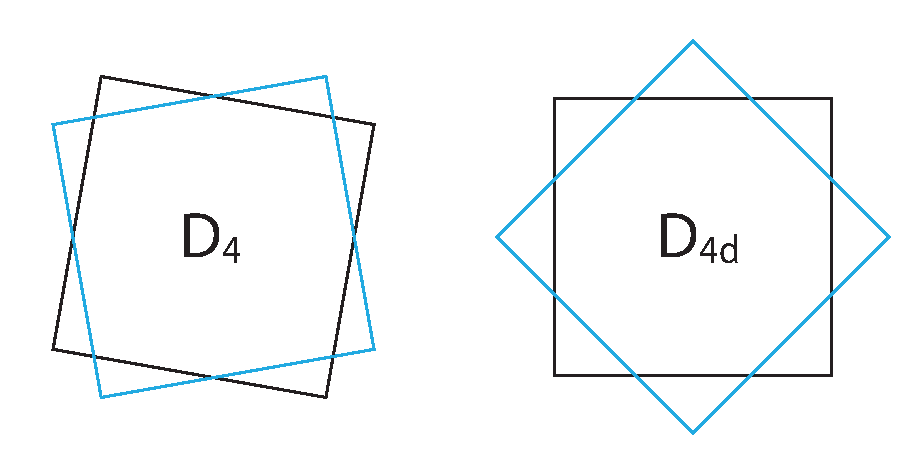
\includegraphics[width=0.78\linewidth]{fig/sketch.pdf}
\end{figure}

\begin{figure}
	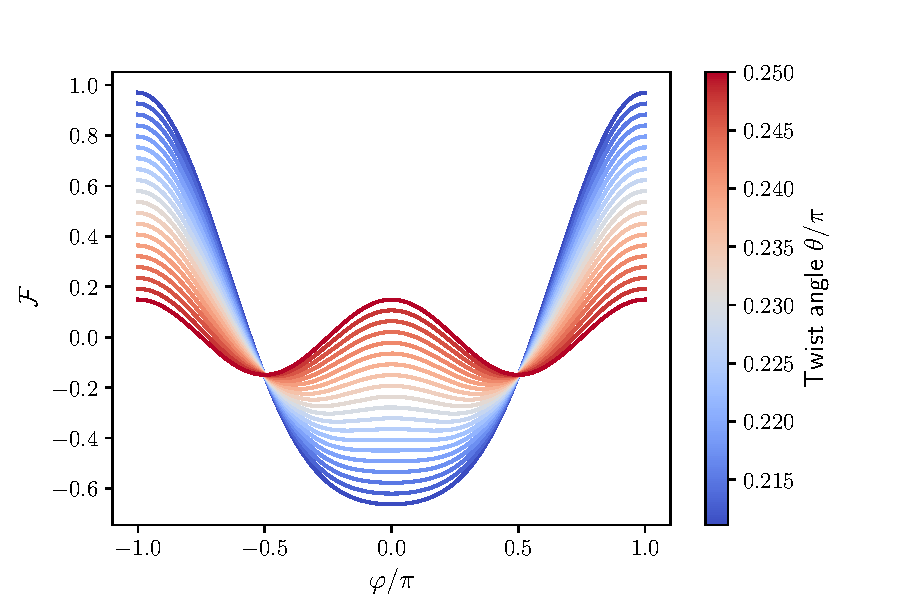
\includegraphics[width=0.78\linewidth]{fig/cos.pdf}
	\caption{\sffamily \, Free energy $\mathcal{F}(\varphi)$ as a function of twist angle $\theta$.}
\label{fig:cos}
\end{figure}


\end{column} % End of the first column


\begin{column}{\sepwid}\end{column} % Empty spacer column

\begin{column}{\onecolwid} % Begin a column (column 2)
\rmfamily
\justify
\begin{block}{Model}


\begin{figure}
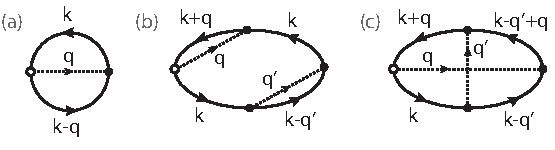
\includegraphics[width=\linewidth]{fig/diagram-figure.pdf}
\caption{\sffamily \,
Diagrammatic expansion of the interlayer current (a) at order $g^2$ and (b-c) at
order $g^4$. Full lines correspond to electronic propagators $G_0$, dashed
lines correspond to impurity vertices paired by disorder average.}
\label{fig:diagram}
\end{figure}

The Hamiltonian of the uncoupled layers is given by
\begin{align}
	\mathcal{H}_0 = \sum_{\mathbf{k}l}\Psi_{\mathbf{k}l}^\dagger
	\left( 
	\xi_{\mathbf{k}} \sigma_z 
	+ \Delta_{\mathbf{k}l}' \sigma_x
	- \Delta_{\mathbf{k}l}'' \sigma_y,
	\right)
	\Psi_{\mathbf{k}l}
\end{align}
with $\xi_\mathbf{k} = \mathbf{k}^2/2m-\mu$ and the superconducting gaps
\begin{align}
	\Delta_{\mathbf{k}1} &= \Delta e^{i\varphi/2} \cos(2\alpha_\mathbf{k} -
	\theta) 
	\nonumber
	\\
	\Delta_{\mathbf{k}2} &= \Delta e^{-i\varphi/2} \cos(2\alpha_\mathbf{k} +
	\theta) \,.
	\label{eq:op}
\end{align}
Here, $\alpha_\mathbf{k}$ is the polar angle and the bilayers are twisted by
$\theta$. The interlayer coupling term is
\begin{align}\label{tun}
	\mathcal{H}' = \sum_{\mathbf{kq}} \gamma_{\mathbf{q}} c_{\mathbf{k},1}^\dagger
	c_{\mathbf{k-q},2} + \textrm{h.c.}
\end{align}
where disorder is captured via a set of Gaussian-distributed random variables $\gamma_\mathbf{q}$ of average $\overline{\gamma_\mathbf{q}}=0$ and variance given by
\begin{align}
	\overline{\gamma_\mathbf{q}^* \gamma_\mathbf{q+p}} &=
	\frac{1}{N}\frac{4\pi g^2}{3\Lambda^2}
	\delta_{\mathbf{p},0}e^{-\mathbf{q}^2/\Lambda^2} \,.
\end{align}
The scale $\Lambda$ defines the momentum non-conservation of the interlayer
tunneling. The model becomes coherent in the limit $\Lambda \rightarrow
0$.

We compute the interlayer current

\begin{align}
	J &= \sum_{\mathbf{kq}} i e^{i\varphi/2}\overline{\gamma_\mathbf{q}
	\langle c_{\mathbf{k},1}^\dagger c_{\mathbf{k-q},2} \rangle} + \textrm{h.c.} 
	\nonumber
	= \text{Tr}
	\left[ \overline{
		j_\mathbf{q} G(\mathbf{k},\mathbf{k-q},\omega_n)}
	\right]
	\label{eq:current}
\end{align}
by a diagrammatic expansion up to fourth order in $g$. 
Here, $G(\mathbf{k},\mathbf{k'},\tau)=\langle T_\tau c_{\mathbf{k}}(\tau) c_{\mathbf{k'}}^\dagger(0) \rangle$ is the full imaginary time ordered Green's function of the disordered system
The $\varphi$-dependence
of the free energy can 
be extracted from the Josephson relation
$J(\varphi)=2\partial \mathcal{F}(\varphi)/\partial \varphi$ and is used to
evaluate the phase diagram of the $\mathcal{T}$-broken phase.


\begin{figure}[t]
	\centering
	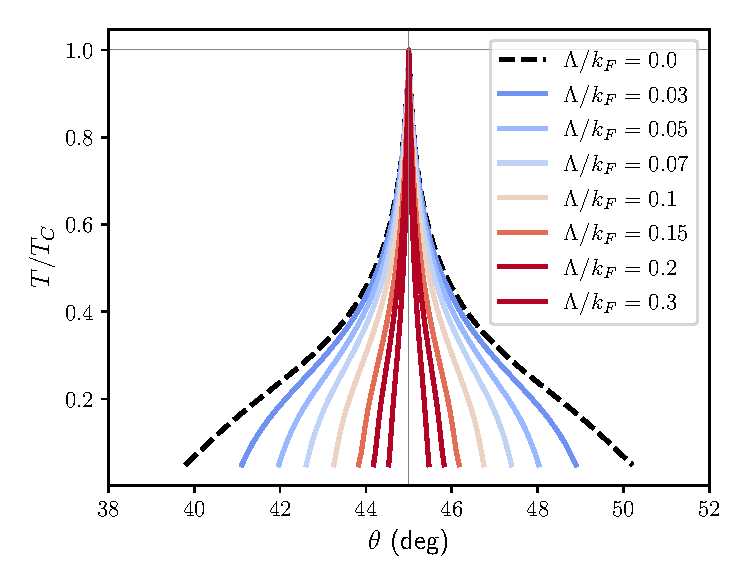
\includegraphics[width=\columnwidth]{fig/phase-diagram.pdf}
	\caption{\sffamily \, Phase diagram of incoherently coupled twisted bilayer cuprates. For a given $\Lambda$, the inside of the cone-shaped region breaks $\mathcal{T}$. Black-dashed lines mark the phase boundary in the clean limit, previously introduced in \cite{Can2021}.}
	\label{fig:phasediagram}
\end{figure}


We confirmed the $\mathcal{T}$-breaking physics of the continuum model by exact
diagonalization of a lattice model with open boundaries of
part of the moire unit cell. This models a realistic electronic structure and 
also captures the effect of Brillouin zone folding.

\begin{figure}
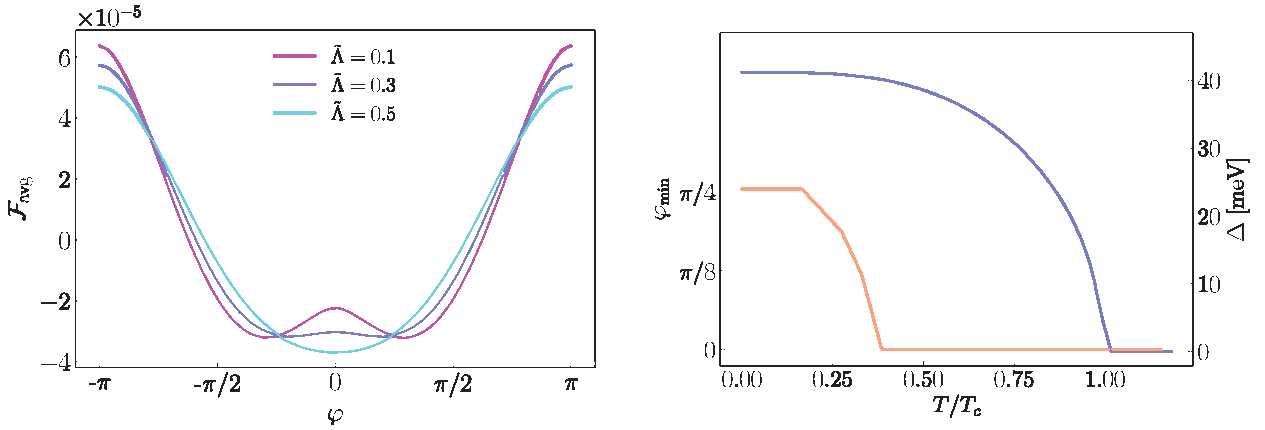
\includegraphics[width=\linewidth]{fig/latt_summ2.pdf}
\caption{\sffamily \,
	Disorder averaged free energy of the bilayer (left) at zero temperature as a
	function of the phase difference. The minima $\varphi_{\rm min}$ are
	situated away from zero at small disorder. Dependence of the
	order parameter amplitude and phase as a function of temperature for
$\tLambda=0.2$ (right).}
\label{fig:tarun}
\end{figure}


\end{block}





\end{column} % End of the second column

\begin{column}{\sepwid}\end{column} % Empty spacer column

\begin{column}{\onecolwid} % The third column




\begin{block}{Topological superconductivity}



\begin{figure}[t]
	\centering
	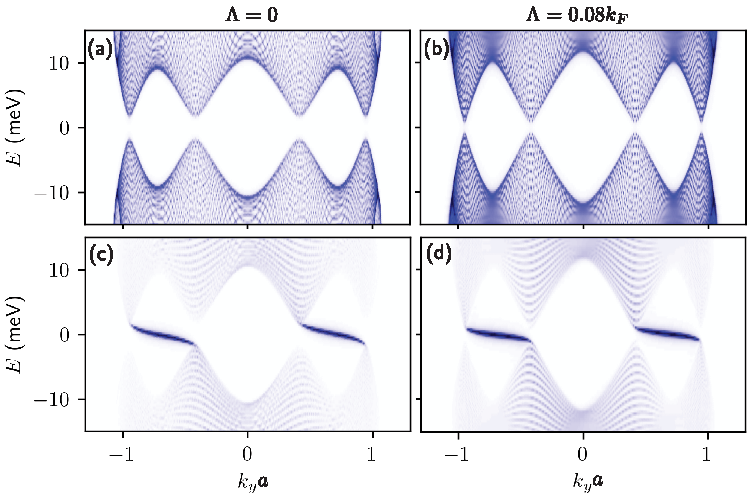
\includegraphics[width=\columnwidth]{fig/spectrum.pdf}
	\caption{\sffamily \, Bulk (a-b) and boundary (c-d) spectrum for incoherently coupled
	cuprate bilayers with $\Lambda=0$ (left) and $\Lambda/k_F=0.08$ (right)
at $45^\circ$ twist angle. The spectrum shows chiral edge modes traversing the
bulk gap indicating a Chern number $\mathcal{C}=4$. }
	\label{fig:edgemode}
\end{figure}

To assess the topological character of the model, we examine the boundary
physics with the surface Green function
\begin{align}
     G_B(x, k_y,\omega_n) &= G(x, k_y) - G(x, k_y) 
     T(k_y)
     G(-x, k_y) 
     \nonumber
     \\
     T(k_y) &= \left[ 
     \frac{1}{\sqrt{N}} \sum_{k_x} G(k_x, k_y)
     \right]^{-1}  \,.
     \label{eq:transfm}
\end{align}
Here, $G$ is the impurity averaged Green function of the coupled cuprate layers
in the Born approximation. The surface spectral function clearly shows edge
modes, indicative of a chiral phase with Chern number $\mathcal{C}=4$.

\vspace{1cm}


\begin{figure}
	\centering
	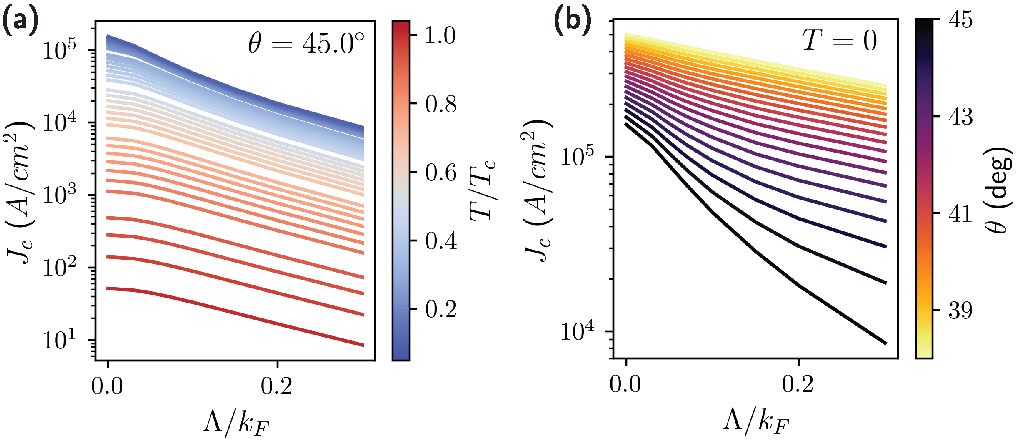
\includegraphics[width=\columnwidth]{fig/jc.pdf}
	\caption{\sffamily \,Critical current $J_c$ of the twisted bilayer as a function as interlayer coherence scale $\Lambda$. Incoherence significantly reduces $J_c$. The color scale denotes temperature $T$ in panel (a) and twist angle $\theta$ in (b).}
	\label{fig:jc}
\end{figure}


\end{block}

%----------------------------------------------------------------------------------------
%	CONCLUSION
%----------------------------------------------------------------------------------------
\begin{block}{Summary}

	We showed that a model of twisted cuprate bilayers with incoherent,
	impurity-mediated, interlayer
tunneling processes gives rise to a broad topological chiral phase around a twist angle
of $45^\circ$ that spontaneously breaks time-reversal symmetry
$\mathcal{T}$.
\end{block}



%----------------------------------------------------------------------------------------
%	REFERENCES
%----------------------------------------------------------------------------------------

\begin{block}{References}

\nocite{*} % Insert publications even if they are not cited in the poster
\small{\bibliographystyle{unsrt}
\bibliography{lit}\vspace{0.75in}}

\end{block}


%----------------------------------------------------------------------------------------

\end{column} % End of the third column

\end{columns} % End of all the columns in the poster

\end{frame} % End of the enclosing frame

\end{document}
